\vspace{20pt}

{\let\clearpage\relax
    \chapter{Нарисуйте граф отношения и постройте матрицу смежности этого графа}}
\begin{tblr}{
    colspec = {X[c,h]X[c]},
    stretch = 0
    }
    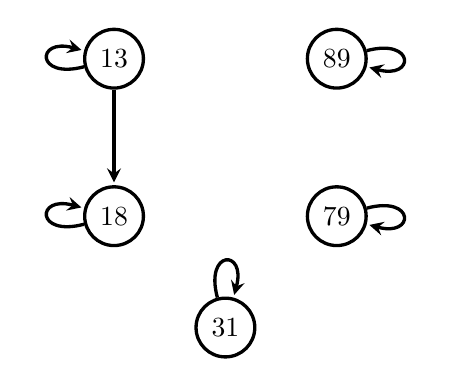
\begin{tikzpicture}[->,>=stealth,auto,shorten >=1pt,very thick,node distance=2cm,main node/.style={circle,draw}]
        \node[main node] (13) {13};
        \node[main node] (18) [below of=13]{18};
        \node[main node] (31) [below right of=18]{31};
        \node[main node] (79) [above right of=31]{79};
        \node[main node] (89) [above of=79]{89};
        \path
        (13) edge node {} (18)
        edge [loop left] node {} (13)
        (18) edge [loop left] node {} (18)
        (31) edge [loop above] node {} (31)
        (79) edge [loop right] node {} (79)
        (89) edge [loop right] node {} (89);
    \end{tikzpicture}
       & {
            \renewcommand{\kbldelim}{(}
            \renewcommand{\kbrdelim}{)}
            $\kbordermatrix{
       & 13 & 18 & 31 & 79 & 89 \\
    13 & 1  & 1  & 0  & 0  & 0  \\
    18 & 0  & 1  & 0  & 0  & 0  \\
    31 & 0  & 0  & 1  & 0  & 0  \\
    79 & 0  & 0  & 0  & 1  & 0  \\
    89 & 0  & 0  & 0  & 0  & 1  \\
                }$
    }                           \\
\end{tblr}
\endinput